\documentclass[12pt]{article} % Sets the font size to 12pt and defines the document as an article

% Packages for mathematical fonts and symbols
\usepackage{amsfonts, amssymb, amsmath}
\usepackage{booktabs}
\usepackage{float}
\usepackage{ulem}
\usepackage{tabularx}
\usepackage[ruled,vlined]{algorithm2e}
\usepackage{graphicx}


% Uncomment the following lines if you want to enable double spacing
%\usepackage{setspace}
%\doublespacing

% Margin settings
\usepackage[margin=1in]{geometry} % Simplifies margin settings using the geometry package

% Header and footer customization
\usepackage{fancyhdr}

\pagestyle{fancy}
\fancyhf{} % Clears default header and footer
\fancyhead[L]{CS250/homework1/JuntangWang} 
\fancyhead[C]{\today} 
\fancyhead[R]{\thepage} 

% Custom commands
\newcommand{\eqn}{\begin{array}{rcl}} % Begin an aligned equation environment
\newcommand{\eqnend}{\end{array}}    % End the aligned equation environment
\newcommand{\qed}{\hfill $\square$} % End of proof symbol

% Title Information
\title{CS521 Homework1} % Replace with your actual title
\author{Juntang Wang}        % Replace with your actual name
\date{\today}             % Automatically uses the current date

\begin{document}

\section{Q1}
\subsection{(a)}
\textbf{Solution:}

\textbf{Step 1: Convert the Hex String to Binary}

First, convert each hex digit to its 4-bit binary equivalent:

\[
\begin{array}{ccccccccc}
\text{Hex:} & 2 & 0 & A & 3 & 0 & 0 & 1 & 2 \\
\text{Bin:} & 0010 & 0000 & 1010 & 0011 & 0000 & 0000 & 0001 & 0010 \\
\end{array}
\]

\textbf{Step 2: Identify the Opcode}

Opcode (bits 31-26): \(001000\). Which corresponds to the \texttt{ADDI} instruction in MIPS.  \cite{MIPS32}

\textbf{Step 3: Break Down the Binary Instruction}

MIPS instructions come in: R-type, I-type, and J-type. Based on the opcode, we can determine the format. The instruction format for I-type (which includes \texttt{ADDI}) is:

\begin{itemize}
    \item \textbf{Opcode (bits 31-26)}: \(001000\) (binary) \(= 8\) (decimal)
    \item \textbf{rs (bits 25-21)}: \(00101\) (binary) \(= \$5\) (register 5)
    \item \textbf{rt (bits 20-16)}: \(00011\) (binary) \(= \$3\) (register 3)
    \item \textbf{Immediate (bits 15-0)}: \(0000000000010010\) (binary) \(= 18\) (decimal)
\end{itemize}



\textbf{Step 4: Assemble the Instruction}

Now, we can construct the instruction:

\[
\boxed{
\texttt{addi \$3, \$5, 18}
}
\quad \text{or} \quad
\boxed{
\texttt{addi \$v1, \$a1, 18}
}
\]


\subsection{(b)}
\textbf{Solution:}

\textbf{Step 1: Identify the Instruction Format}

The instruction is \texttt{sw \$9, 4(\$2)}. This is a \emph{store word} instruction, which is an \textbf{I-type} instruction in MIPS. The I-type instruction format is:
\[
\text{[opcode (6 bits)]\quad[rs (5 bits)]\quad[rt (5 bits)]\quad[immediate (16 bits)]}
\]

\textbf{Step 2: Determine the Opcode and Register Numbers}

\begin{itemize}
    \item \textbf{Opcode}: The opcode for \texttt{sw} is \(43\) in decimal, which is \(101011\) in binary.\cite{MIPS32}
    \item \textbf{rs} (\emph{base register}): \(\$2\) corresponds to register number \(2\). In binary: \(00010\).
    \item \textbf{rt} (\emph{source register}): \(\$9\) corresponds to register number \(9\). In binary: \(01001\).
    \item \textbf{Immediate}: The offset is \(4\). In 16-bit binary: \(0000\ 0000\ 0000\ 0100\).
\end{itemize}

\textbf{Step 3: Assemble the Binary Instruction}

Concatenating these fields, we get the 32-bit instruction:
\[
\begin{array}{rl}
\text{Instruction Binary}: & 1\ 0\ 1\ 0\ 1\ 1\ 0\ 0\ 0\ 1\ 0\ 0\ 1\ 0\ 0\ 1\ 0\ 0\ 0\ 0\ 0\ 0\ 0\ 0\ 0\ 0\ 0\ 1\ 0\ 0 \\
\end{array}
\]

\textbf{Step 4: Group the Bits and Convert to Hexadecimal}

We will group the 32 bits into 8 groups of 4 bits, starting from bit 31 down to bit 0:
\[
\begin{array}{llcl}
\text{Group} & \text{Bits (from bit positions)} & \text{Binary} & \text{Hex} \\
\hline
\text{1} & \text{Bits 31--28} & 1\ 0\ 1\ 0 & \texttt{A} \\
\text{2} & \text{Bits 27--24} & 1\ 1\ 0\ 0 & \texttt{C} \\
\text{3} & \text{Bits 23--20} & 0\ 1\ 0\ 0 & \texttt{4} \\
\text{4} & \text{Bits 19--16} & 1\ 0\ 0\ 1 & \texttt{9} \\
\text{5} & \text{Bits 15--12} & 0\ 0\ 0\ 0 & \texttt{0} \\
\text{6} & \text{Bits 11--8} & 0\ 0\ 0\ 0 & \texttt{0} \\
\text{7} & \text{Bits 7--4} & 0\ 0\ 0\ 0 & \texttt{0} \\
\text{8} & \text{Bits 3--0} & 0\ 1\ 0\ 0 & \texttt{4} \\
\end{array}
\]

\textbf{Step 5: Write the Hexadecimal Representation}

Combining the hexadecimal digits from each group:
\[
\boxed{\texttt{0xAC490004}}
\]



\section{Q2}
\subsection{(a)}
\textbf{Solution:}

\textbf{(a) Instruction Count}

In this part, we are asked to count the number of instructions, excluding labels and non-instruction directives. We will count the number of instructions both with and without including \texttt{nop} instructions, as they are actual instructions but do not perform any operation.

\begin{itemize}
    \item \textbf{-O0 (Unoptimized version)}:
    \begin{itemize}
        \item Total lines: 57 lines (from line 6 to line 62)
        \item With \texttt{nop}: There are a total of $\boxed{\textbf{57 instructions}}$.
        \item \sout{Without \texttt{nop}: There are \textbf{50 instructions} \text{(excluding 7 \texttt{nop} instructions)}.}
    \end{itemize}
    
    \item \textbf{-O3 (Optimized version)}:
    \begin{itemize}
        \item Total lines: 32 lines (from line 2 to line 33)
        \item With \texttt{nop}: There are a total of $\boxed{\textbf{32 instructions}}$.
        \item \sout{Without \texttt{nop}: There are \textbf{32 instructions} \text{(since there are no \texttt{nop})}.}
    \end{itemize}
\end{itemize}


\subsection{(b)}
\textbf{Solution:}

\begin{itemize}

\item \textbf{Memory Access Instructions:} 

In MIPS, \textbf{memory access} instructions are typically the following\footfullcite{MIPS32}:
\begin{itemize}
    \item \texttt{lw} (load word): Loads a value from memory into a register.
    \item \texttt{sw} (store word): Stores a value from a register into memory.
    \item \sout{\texttt{andi} (AND immediate): Used for bitwise operations but does not access memory.}
    \item \sout{\texttt{sll} (shift left logical): Used for shifting bits but does not access memory.}
    \item \sout{\texttt{sra} (shift right arithmetic): Used for shifting bits but does not access memory.}
    \item \sout{\texttt{lui} (load upper immediate): Load the upper part of an address but does not access memory.}
\end{itemize}

\item \textbf{Memory Access Instructions in O0:}

\begin{enumerate}
    \tiny
    \item \texttt{sw \$fp, 4(\$sp)} (line 7) \\
    \textbf{Memory access}: Stores the value of \texttt{\$fp} into memory.

    \item \texttt{lw \$2, \%lo(m\_z)(\$2)} (line 10) \\
    \textbf{Memory access}: Loads the value from memory into register \texttt{\$2}.

    \item \texttt{lw \$2, \%lo(m\_z)(\$2)} (line 26) \\
    \textbf{Memory access}: Loads the value from memory into register \texttt{\$2}.

    \item \texttt{sw \$3, \%lo(m\_z)(\$2)} (line 31) \\
    \textbf{Memory access}: Stores the value from register \texttt{\$3} into memory.

    \item \texttt{lw \$2, \%lo(m\_w)(\$2)} (line 33) \\
    \textbf{Memory access}: Loads the value from memory into register \texttt{\$2}.

    \item \texttt{lw \$2, \%lo(m\_w)(\$2)} (line 44) \\
    \textbf{Memory access}: Loads the value from memory into register \texttt{\$2}.

    \item \texttt{sw \$3, \%lo(m\_w)(\$2)} (line 49) \\
    \textbf{Memory access}: Stores the value from register \texttt{\$3} into memory.

    \item \texttt{lw \$2, \%lo(m\_z)(\$2)} (line 51) \\
    \textbf{Memory access}: Loads the value from memory into register \texttt{\$2}.

    \item \texttt{lw \$2, \%lo(m\_w)(\$2)} (line 55) \\
    \textbf{Memory access}: Loads the value from memory into register \texttt{\$2}.

    \item \texttt{lw \$fp, 4(\$sp)} (line 59) \\
    \textbf{Memory access}: Loads the value from memory into register \texttt{\$fp}.
\end{enumerate}

\begin{itemize}
    \item \texttt{lw} (load word) instructions: 7 instances.
    \item \texttt{sw} (store word) instructions: 3 instances.
    \item In total: $7 + 3 = \boxed{10}$
\end{itemize}

\item \textbf{Memory Access Instructions in the O3:}

\begin{enumerate}
    \tiny
    \item \texttt{lw \$7, \%lo(m\_z)(\$9)} (line 3) \\
    \textbf{Memory access}: Loads the value from memory into register \texttt{\$7}.

    \item \texttt{lw \$6, \%lo(m\_w)(\$8)} (line 8) \\
    \textbf{Memory access}: Loads the value from memory into register \texttt{\$6}.

    \item \texttt{sw \$2, \%lo(m\_w)(\$8)} (line 30) \\
    \textbf{Memory access}: Stores the value from register \texttt{\$2} into memory.

    \item \texttt{sw \$3, \%lo(m\_z)(\$9)} (line 31) \\
    \textbf{Memory access}: Stores the value from register \texttt{\$3} into memory.
\end{enumerate}

\begin{itemize}
    \item \texttt{lw} (load word) instructions: 2 instances.
    \item \texttt{sw} (store word) instructions: 2 instances.
    \item In total: $2 + 2 = \boxed{4}$
\end{itemize}

\end{itemize}
\subsection{(c)}
\textbf{Solution:}

\textbf{Mapping of Unoptimized and Optimized Code to C Source}

The difference between the unoptimized (`-O0`) and optimized (`-O3`) code lies in how assembly instructions map to the original C code.

\begin{itemize}
    \item \textbf{-O0 (Unoptimized version)}:
    \begin{itemize}
        \item The unoptimized version follows a $\boxed{\textbf{“block”}}$ pattern, where each C statement corresponds directly to a set of assembly instructions.
        \item Each block of C code generates a block of assembly instructions, often including redundant instructions like `nop`. The instructions are laid out in sequence, matching the C code line by line, making it easy to trace but resulting in verbose and inefficient code.
    \end{itemize}

    \item \textbf{-O3 (Optimized version)}:
    \begin{itemize}
        \item The optimized version exhibits a $\boxed{\textbf{“stripe”}}$ pattern, where assembly instructions correspond to multiple lines of C code.
        \item The compiler optimizes by reordering, combining, or eliminating instructions. This leads to assembly instructions serving multiple parts of the C code, reducing redundancy and improving efficiency. As a result, the mapping is more scattered (stripes) and less direct, making it harder to trace.
    \end{itemize}
\end{itemize}
\subsection{(d)}
\textbf{Solution:}

\textbf{General Strategies Taken by the Optimizer}

Based on the comparison between unoptimized (`-O0`) and optimized (`-O3`) code, we can infer several general strategies that the optimizer uses to improve performance:

\begin{itemize}
    \item \textbf{Fewer Instructions:}
    The optimized version has significantly fewer lines of assembly code compared to the unoptimized version. This reduction is achieved by removing redundant instructions, such as \texttt{nop}, and optimizing the code to perform the same tasks with fewer operations, resulting in more efficient execution.

    \item \textbf{Reduced Memory Access:}
    The optimized code makes fewer memory accesses by using registers more effectively (register allocation). By minimizing unnecessary load and store operations, the optimizer reduces the overhead of accessing slower memory resources, which improves performance.

    \item \textbf{Instruction Optimization:}
    The optimizer improves instruction execution through techniques like instruction reordering. By rearranging instructions to minimize stalls, hazards, and dependencies, it allows for more efficient use of the CPU. This optimization is reflected in the "striped" pattern of the optimized assembly code, where instructions correspond to multiple lines of C code instead of following a direct, line-by-line mapping.
\end{itemize}
\subsection{(e)}
For this part of the homework, I have included an illustration of a platypus. The image was generated using the DALL-E tool by OpenAI, based on a textual description provided.

\begin{figure}[htbp]
    \centering
    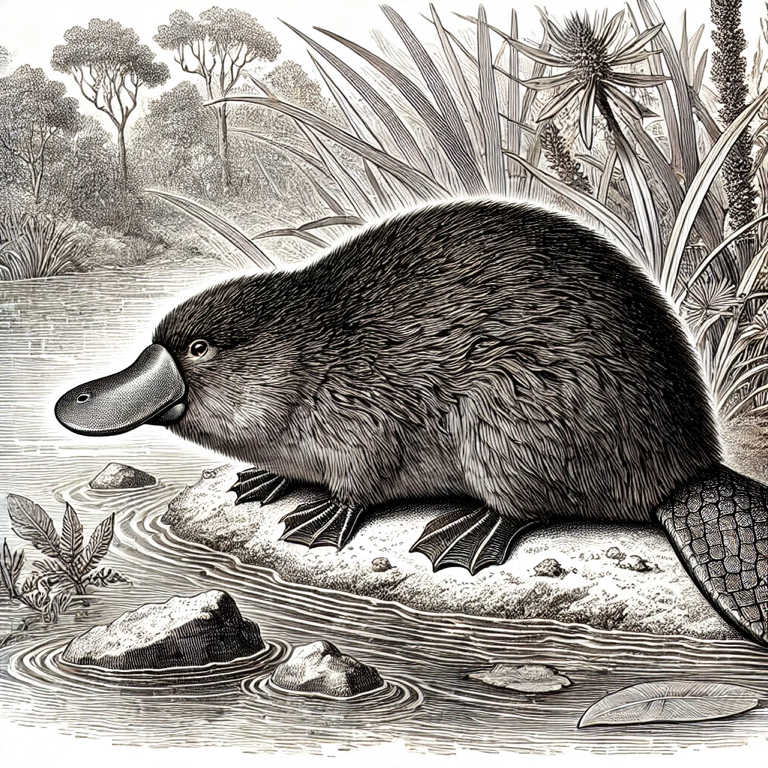
\includegraphics[width=0.38\textwidth]{figures/playtus.png}
    \caption{Platypus illustration generated using AI (DALL-E)\cite{openai2024platypus}.}
\end{figure}



\bibliography{CS250}
\bibliographystyle{IEEEtran}

\end{document}
